\begin{center}
	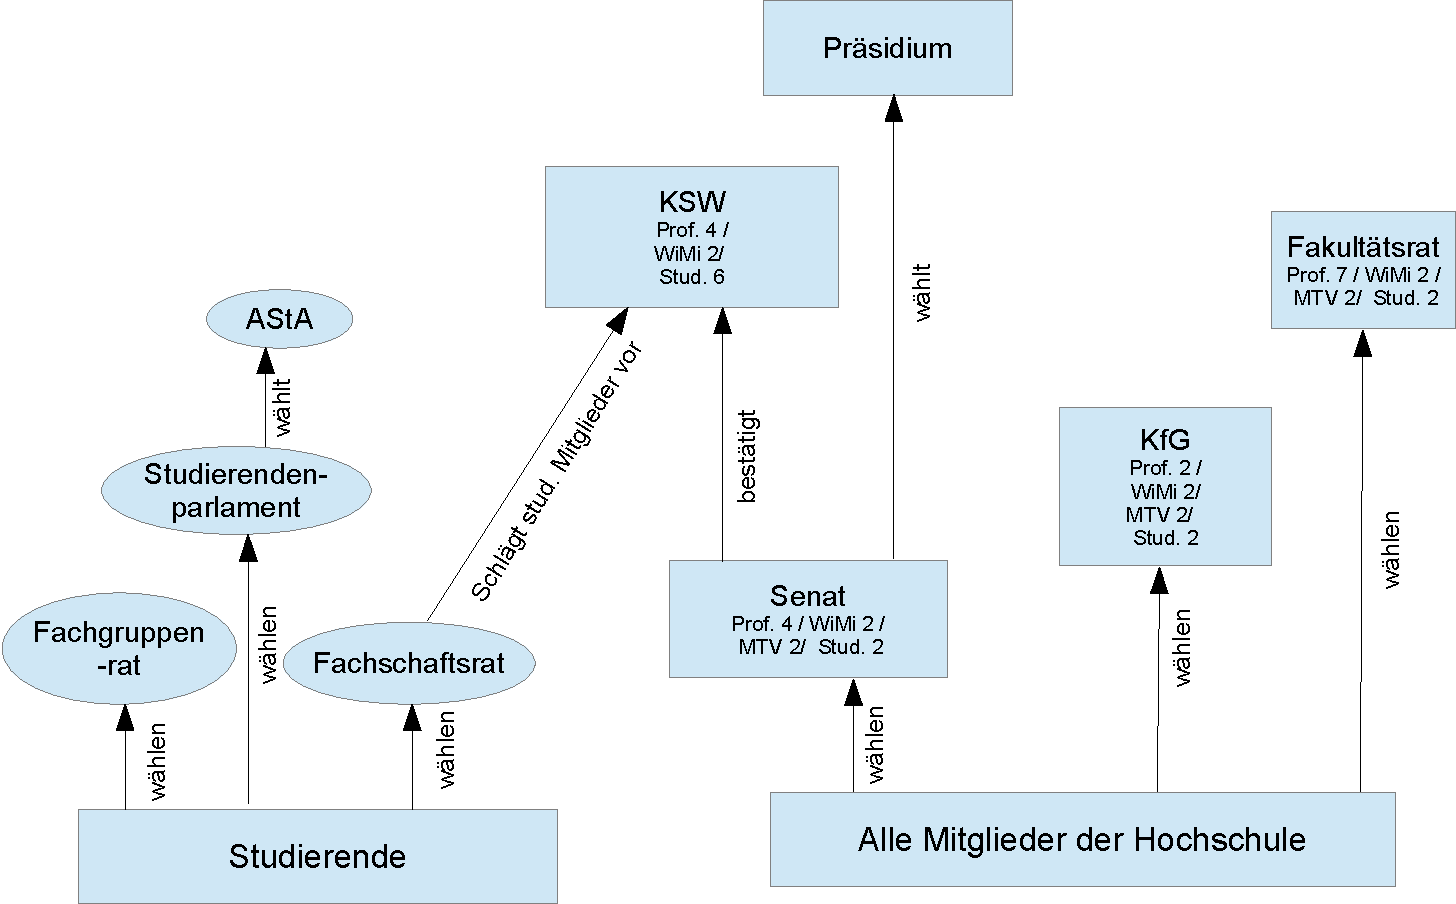
\includegraphics[angle=90]{bilder/gremienkunde3}
\end{center}
\newpage
\subsection{Fachgruppe}
	\label{fachgruppe}
%	\url{http://fginfo.cs.tu-bs.de}
	Die Fachgruppe seid ihr! Die Fachgruppe aus allen Studierenden der Fachrichtung Informatik. Diese wählen einen Fachgruppenrat, der sich dann für die Interessen aller einsetzt. 
	Im Fachgruppenraum IZ150 stehen dir jederzeit zuverlässige Mitstudierende zur Verfügung, denen du Fragen bezüglich deines Studiums und allem drumherum stellen kannst. Einige sind Mitglieder des Fachgruppenrats und dafür verantwortlich, die Meinungen aller Informatikstudierenden gegenüber der Fakultät und in verschiedenen Kommissionen zu vertreten. Eine richtige Trennung zwischen Fachgruppenrat und Fachgruppe besteht bei uns nicht. Also komm vorbei, bringt dich ein und engagier dich für unsere Studienrichtung oder hol dir einfach ein paar koffeinreiche Erfrischungen. 
